\documentclass[sigchi, review]{acmart}

\usepackage{booktabs} % For formal tables


% Copyright
%\setcopyright{none}
%\setcopyright{acmcopyright}
%\setcopyright{acmlicensed}
%\setcopyright{rightsretained}
%\setcopyright{usgov}
%\setcopyright{usgovmixed}
%\setcopyright{cagov}
\setcopyright{licensedcagov}
%\setcopyright{cagovmixed}
%\setcopyright{licensedothergov}

% DOI
\acmDOI{10.475/123_4}

% ISBN
\acmISBN{123-4567-24-567/08/06}

%Conference
\acmConference[WOODSTOCK'97]{ACM Woodstock conference}{July 1997}{El
  Paso, Texas USA}
\acmYear{1997}
\copyrightyear{2016}

\acmPrice{15.00}


\begin{document}
\title{SIG Proceedings Paper in LaTeX Format}
\titlenote{Produces the permission block, and
  copyright information}
\subtitle{Extended Abstract}
\subtitlenote{The full version of the author's guide is available as
  \texttt{acmart.pdf} document}

\author{Ben Trovato}
\authornote{Dr.~Trovato insisted his name be first.}
\orcid{1234-5678-9012}
\affiliation{%
  \institution{Institute for Clarity in Documentation}
  \streetaddress{P.O. Box 1212}
  \city{Dublin}
  \state{Ohio}
  \postcode{43017-6221}
}
\email{trovato@corporation.com}

\author{G.K.M. Tobin}
\authornote{The secretary disavows any knowledge of this author's actions.}
\affiliation{%
  \institution{Institute for Clarity in Documentation}
  \streetaddress{P.O. Box 1212}
  \city{Dublin}
  \state{Ohio}
  \postcode{43017-6221}
}
\email{webmaster@marysville-ohio.com}

\author{Lars Th{\o}rv{\"a}ld}
\authornote{This author is the
  one who did all the really hard work.}
\affiliation{%
  \institution{The Th{\o}rv{\"a}ld Group}
  \streetaddress{1 Th{\o}rv{\"a}ld Circle}
  \city{Hekla}
  \country{Iceland}}
\email{larst@affiliation.org}

\author{Valerie B\'eranger}
\affiliation{%
  \institution{Inria Paris-Rocquencourt}
  \city{Rocquencourt}
  \country{France}
}
\author{Aparna Patel}
\affiliation{%
 \institution{Rajiv Gandhi University}
 \streetaddress{Rono-Hills}
 \city{Doimukh}
 \state{Arunachal Pradesh}
 \country{India}}
\author{Huifen Chan}
\affiliation{%
  \institution{Tsinghua University}
  \streetaddress{30 Shuangqing Rd}
  \city{Haidian Qu}
  \state{Beijing Shi}
  \country{China}}

\author{Charles Palmer}
\affiliation{%
  \institution{Palmer Research Laboratories}
  \streetaddress{8600 Datapoint Drive}
  \city{San Antonio}
  \state{Texas}
  \postcode{78229}}
\email{cpalmer@prl.com}

\author{John Smith}
\affiliation{\institution{The Th{\o}rv{\"a}ld Group}}
\email{jsmith@affiliation.org}

\author{Julius P.~Kumquat}
\affiliation{\institution{The Kumquat Consortium}}
\email{jpkumquat@consortium.net}

% The default list of authors is too long for headers.
\renewcommand{\shortauthors}{B. Trovato et al.}


\begin{abstract}
This paper provides a sample of a \LaTeX\ document which conforms,
somewhat loosely, to the formatting guidelines for
ACM SIG Proceedings.
\end{abstract}

%
% The code below should be generated by the tool at
% http://dl.acm.org/ccs.cfm
% Please copy and paste the code instead of the example below.
%
\begin{CCSXML}
<ccs2012>
 <concept>
  <concept_id>10010520.10010553.10010562</concept_id>
  <concept_desc>Computer systems organization~Embedded systems</concept_desc>
  <concept_significance>500</concept_significance>
 </concept>
 <concept>
  <concept_id>10010520.10010575.10010755</concept_id>
  <concept_desc>Computer systems organization~Redundancy</concept_desc>
  <concept_significance>300</concept_significance>
 </concept>
 <concept>
  <concept_id>10010520.10010553.10010554</concept_id>
  <concept_desc>Computer systems organization~Robotics</concept_desc>
  <concept_significance>100</concept_significance>
 </concept>
 <concept>
  <concept_id>10003033.10003083.10003095</concept_id>
  <concept_desc>Networks~Network reliability</concept_desc>
  <concept_significance>100</concept_significance>
 </concept>
</ccs2012>
\end{CCSXML}

\ccsdesc[500]{Computer systems organization~Embedded systems}
\ccsdesc[300]{Computer systems organization~Redundancy}
\ccsdesc{Computer systems organization~Robotics}
\ccsdesc[100]{Networks~Network reliability}


\keywords{ACM proceedings, \LaTeX, text tagging}

\begin{teaserfigure}
  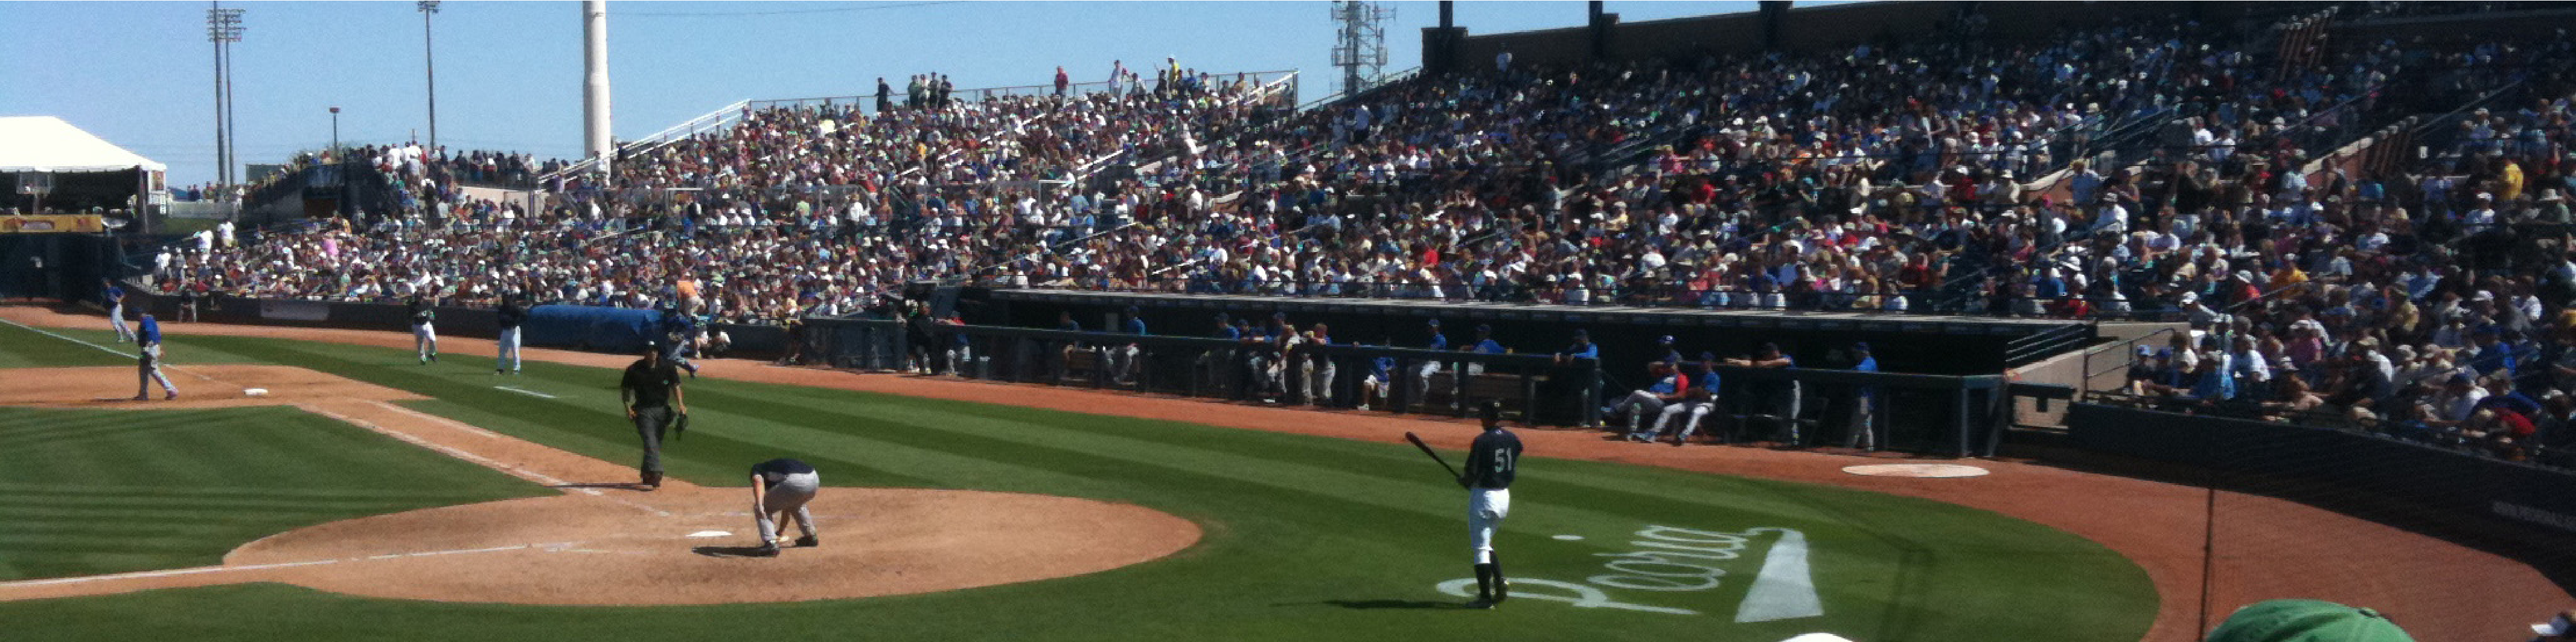
\includegraphics[width=\textwidth]{sampleteaser}
  \caption{This is a teaser}
  \label{fig:teaser}
\end{teaserfigure}


\maketitle

\section{Motivation and Research Problem}

While advances in antiretroviral therapy (ART) have substantially reduced AIDS-related morbidity and mortality, successful therapy requires sustained ART adherence for 1) HIV viral suppression, 2) decreasing the risk of developing antiretroviral (ARV) drug resistance, 3) improving immunological and clinical outcomes resulting in increased survival and improved quality of life and 4) reducing the risk of transmitting HIV (World Health Organization.,  2003;Chesney,  2006). Non-adherence has been associated with increased rate of hospitalization and longer hospital stays, that adds to the economic burden of an already overburdened healthcare system (Protopopescu et al. 2009). Transmission of drug resistant HIV (TDR) can also emerge from non-adherence. In the United States, several studies of different groups of HIV-positive individuals generally show similar, suboptimal rates of adherence. The goal of this pilot study is to assess whether a medication event monitoring systems (MEMS) along with a smartphone gamified app with a competitive element can enhance the medication adherence of non-adherent HIV patients with detectable viral load.

\section{Background Literature}

Current research on improving ART adherence has used a variety of methods to assess ART adherence including: 1) MEMS and variants of it (including special pill bottles with sensors in bottles), 2) pill count, and 3) self-report, 4) pharmacy refill data (Achieng et al. 2013), and 5) biological markers, such as HIV viral load and drug concentration in hair (Gandhi et al. 2009). While previous studies of MEMS - a conventional medicine container fitted with a special closure that records the time and date of each time the container is opened and closed, have been conducted with HIV/AIDS patients, we are not aware of any studies that have used competitive gaming with social media to promote ART adherence. Our proposed technology intervention is unique and innovative in that it consists of a competitive game delivered through a mobile app on patient smartphones that provides information on ART adherence performance of the entire intervention group to individual patients in the intervention group. This competitive game is used in conjunction with a “passive” MEMS system (medication pill bottles with smart caps and NFC enabled smartphone) to only capture information on ART adherence (time and date of the taking of medicine) of enrolled patients unobtrusively without reminding patients with aural or visual cues for taking their medicine. We posit that the competitive gaming intervention can enhance ART adherence in a sample of poorly ART adherent HIV/AIDS patients. The proposed study is rooted in the Health Belief Model, a widely cited model of preventive health behavior that proposes that a “cue to action” for a patient elicits health behavior change in the patient (Rosenstock et al. 1988).

\section{Methods}

20 patients with detectable viral load have been recruited for this four-month long pilot study from the Immunodeficiency Clinic at the Erie County Medical Center in Buffalo, New York, and have been assigned equally to the intervention and control groups. The study consists of three phases including baselining (MEMS technology for both control and intervention patients), intervention (game app is added for intervention patients), and habit (game app is withdrawn). All patients have been supplied with one or more MEMS-enabled medication pill bottles with smart caps (one pill bottle per medicine) along with a smartphone and have been asked to swipe or scan their smartphone on top of the smart cap of the pill bottle after taking their medicine. The MEMS app provided on the smartphones captures and transmits the pill consumption data along with smart cap id and date/time of swiping to our cloud, and this daily data will be captured throughout the four-month study. The intent behind the one-month baselining phase is to establish an individual baseline of ART adherence for each patient in the study. Each day during the two-month long intervention phase, the aggregate ART adherence performance for the entire intervention group for the previous day will also be calculated and sent as feedback through the gamification app only to the intervention group patients. This performance information will include the number of patients in the intervention group who were fully adherent (took all meds/doses as prescribed), partially adherent (took some meds/doses but not all as prescribed), and not adherent (took no meds/doses as prescribed) the previous day. During the one-month long habit phase, we will stop sending aggregate ART adherence information to the intervention group patients. We have three main data sources for analyses – patient electronic medical record (EMR) for co-morbid conditions, our cloud setup for daily MEMS usage data, and four surveys for self-reported data on a variety of psychological, perceptual, behavioral, and demographic variables. The data on daily MEMS usage will be used to operationalize adherence. The survey and EMR data will be used to operationalize the independent and control variables. Outcome variables viral load and ARV drug concentration are measured at enrollment and at the end of each month. Viral load will be obtained from Plasma HIV-1 RNA (pVL) quantification using blood samples. ARV drug concentration will be obtained using state-of-the-art LC-MS/MS techniques from patient blood and hair samples.

\section{Expected Results}

(1) The proposed competitive game intervention delivered through a mobile app on patient smartphones should improve three specific patient outcomes over and above those achieved through the passive MEMS intervention alone. These three outcomes include: a) ART adherence; b) viral load; and c) drug concentration in blood serum and hair samples. (2) ART adherence habits are formed as a result of the proposed competitive game intervention during game withdrawal period (3) MEMS technology is validated through high correlation between drug concentration and the drug adherence captured through MEMS use (4) Demographic (e.g., age, gender, ethnicity), clinical (co-morbid conditions, source of HIV, ART regimen), and psychological (HIV treatment adherence self-efficacy) act as moderators of the relationship between the technology interventions and patient outcomes. 

\section{Implications}

We believe that our proposed study will, therefore, open a new research trajectory in the ART adherence field. If our hypotheses are borne out in this study, validation with larger sample sizes will be warranted; and, a cost-benefit analysis will become necessary. Assuming positive results, the usage of a passive MEMS that is used alone or in conjunction with a competitive game should then be evaluated as a standard of care in the population of poorly adherent HIV/AIDS patients. If positive results are subsequently validated, then the proposed technology intervention focused on enhancing ART adherence through fun and competition could significantly enhance the standard of care for with respect to poorly adherent HIV/AIDS patients. This change in clinical practice may also have broader implications for the self-management of other chronic diseases as well.\cite{kennedy2015pocket}

\bibliographystyle{ACM-Reference-Format}
\bibliography{sample-bibliography}

\end{document}
